% Original book diagram: fig:cv_pipeline
% Book source: sections/Part_V/CV.tex
% Original diagram authorship retained. Visual design: Ziad Mosalam.
\documentclass[11pt,border=8pt]{standalone}
\usepackage{amsmath,amssymb,graphicx,tikz}
\usetikzlibrary{arrows.meta,automata,positioning,calc,shapes.geometric,fit,backgrounds,patterns}
\newcommand{\vect}[1]{\mathbf{#1}}
\newcommand{\mat}[1]{\mathbf{#1}}
\newcommand{\Normal}{\mathcal{N}}
\newcommand{\prob}{p}
\newcommand{\E}{\mathbb{E}}
\newcommand{\Var}{\mathrm{Var}}
\newcommand{\Cov}{\mathrm{Cov}}
\newcommand{\CovP}{\mathbf{P}}
\newcommand{\Prob}{\mathbb{P}}
\setlength{\textwidth}{6.5in}
% Shared visual vocabulary for the book's original diagrams.
% Figures opt in explicitly, so unrelated text and existing additions are unchanged.
\definecolor{BookBlue}{HTML}{003262}
\definecolor{BookGold}{HTML}{B17A00}
\definecolor{BookTeal}{HTML}{247C86}
\definecolor{BookInk}{HTML}{30363B}
\definecolor{BookLight}{HTML}{E9EFF5}
\tikzset{
  book figure/.style={font=\small\rmfamily, color=BookBlue, text=BookInk,
    line width=0.8pt, >=Latex},
  book axis/.style={->, draw=BookInk, line width=0.6pt},
  book link/.style={->, draw=BookBlue, line width=0.8pt},
  book observation/.style={draw=BookGold, fill=BookGold!8},
  book state/.style={draw=BookBlue, fill=BookLight},
  book note/.style={font=\footnotesize\rmfamily, text=BookInk}
}

\begin{document}
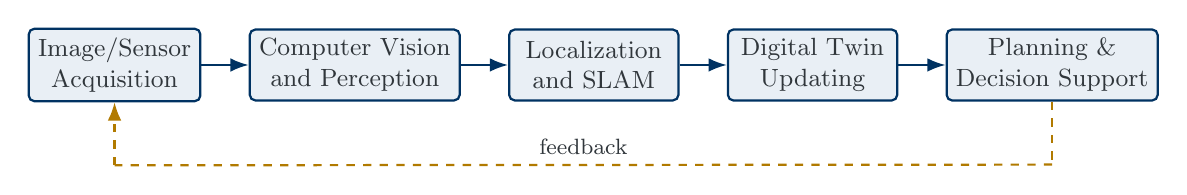
\begin{tikzpicture}[book figure,
    node distance=1.35cm and 0.6cm,
    >=Latex,
    every node/.style={align=center, font=\small},
    block/.style={
        rectangle,
        rounded corners=2pt,
        draw,
        minimum width=2.15cm,
        minimum height=0.9cm,
        line width=0.8pt,
        fill=BookLight
    },
    arrow/.style={->, draw=BookBlue, line width=0.8pt},
    feedback/.style={->, draw=BookGold, dashed, line width=0.8pt}
]

\node[block] (sense) {Image/Sensor\\Acquisition};
\node[block, right=of sense] (vision) {Computer Vision\\and Perception};
\node[block, right=of vision] (slam) {Localization\\and SLAM};
\node[block, right=of slam] (dt) {Digital Twin\\Updating};
\node[block, right=of dt] (decision) {Planning \&\\Decision Support};

\draw[arrow] (sense) -- (vision);
\draw[arrow] (vision) -- (slam);
\draw[arrow] (slam) -- (dt);
\draw[arrow] (dt) -- (decision);

% feedback loop: vertical down, horizontal left, vertical up
\draw[dashed, draw=BookGold, line width=0.8pt]
(decision.south) -- ([yshift=-8mm]decision.south);

\draw[dashed, draw=BookGold, line width=0.8pt]
([yshift=-8mm]decision.south) --
node[midway, above, font=\footnotesize]{feedback}
([yshift=-8mm]sense.south);

\draw[feedback]
([yshift=-8mm]sense.south) -- (sense.south);

\end{tikzpicture}
\end{document}
